\documentclass[11pt, oneside]{article}   	% use "amsart" instead of "article" for AMSLaTeX format

\usepackage{}
%\geometry{landscape}                		% Activate for for rotated page geometry
%\usepackage[parfill]{parskip}    		% Activate to begin paragraphs with an empty line rather than an indent
\usepackage{graphicx}				% Use pdf, png, jpg, or eps� with pdflatex; use eps in DVI mode
								% TeX will automatically convert eps --> pdf in pdflatex		
\usepackage{amssymb}

\usepackage{ifpdf}
\ifpdf
   \pdfcompresslevel=9
   \pdfpagewidth=8.5 true in
   \pdfpageheight=11 true in
   \pdfhorigin=1 true in
   \pdfvorigin=1.25 true in
\fi



\textwidth=6.50in
\textheight=9.00in
\topmargin=0.0in
\headsep=0.0in
\headheight=0.0in
\oddsidemargin=0.0in
\evensidemargin=0.0in




\begin{document}

\section{Scalable Node Manager}

The node manager is a key component in the ESGF node software stack that gathers metrics,     The present implementation of the node manager has scalability limitations arising from  the peer-to-peer protocol.  We are redesigning the node manager to correct existing limitations in consistent reporting of information and address these scalability limitation.  Our design centers on use of communication patterns that incorporate both hierarchal and peer-to-peer organization.  We introduce the concept of super nodes, which do additional heavy lifting for the node manager functionality.  Additionally, other nodes will have the capability to assume a supernode role given failure of original super nodes.  The next-generation node manager will provide a consistent store, which should enable coordination of activities or failover capability for additional ESGF software components beyond the several that rely on the node manager presently.  Moreover, we will support current components such as the dashboard by providing a registration.xml. 

The design phase for the node manager is still in progress.  We expect to complete it and elicit feedback from the community.   In the meantime, we can prototype several of the key node manager functions, such as communication protocols for health check and supernode failure.  We plan to rely on django services so their integration with the current software stack is key to a successful deployment.  Given that, we can plan on a deployment roadmap for existing esgf nodes.   We anticipate making considerable implementation progress in 2015 and should have testable code deployed to nodes by the years close.
\begin{center}
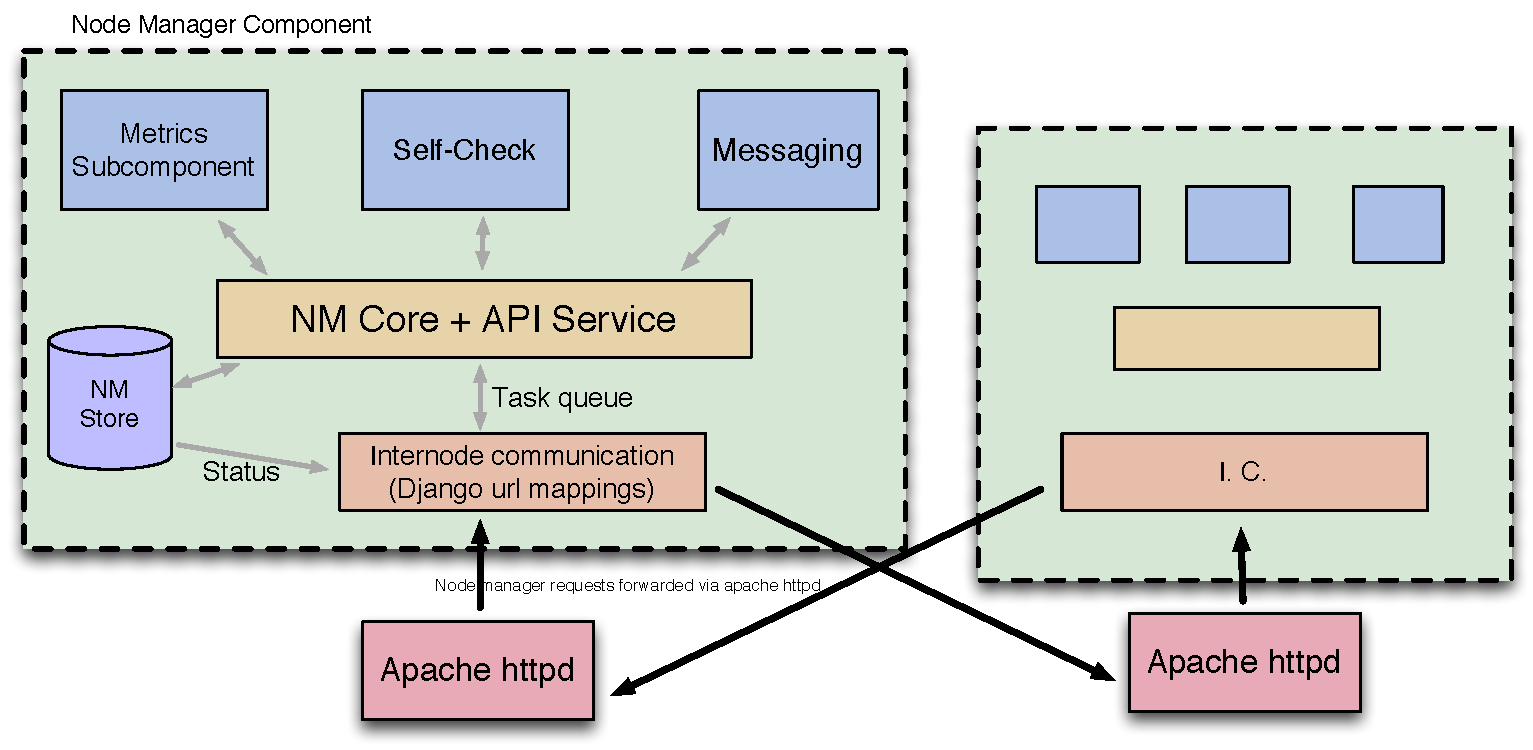
\includegraphics[width=5.5in]{../presentation/NM-design-v2.pdf}
\end{center}

\begin{tabular}{ll}
\hline
\textbf{Expected Time of Achievment} & \textbf{Milestones} \\
\hline
February 2015 & Design to community for feedback \\
March 2015 & Receive and incorporate design feedback \\
July 2015 & Full alpha version completed in test environment \\
September 2015  & Alpha version tested at select sites \\
December 2015 &  Beta version tested at additional sites \\
\end{tabular} 
\end{document}  